\section{Rheologie}
\label{Kapitel:Rheologie}
Rheologie ist die Wissenschaft über das Verhalten von Stoffen unter Einfluss äusserer Kräfte. Es wird untersucht wie Festkörper, Flüssigkeiten und Gase reagieren wenn sie deformiert werden.\\
Diese Arbeit beschäftigt sich mit der Simulation von Flüssigmörteln, weshalb hier nicht weiter auf Festkörper und Gase eingangen wird. \todo{Quellen}

\todo{Zitat Entfernen}\cite{boehme}
\subsection{Massen- und Impulserhaltung}
Die Massen- und Impulserhaltungsgleichung eines inkompressiblen Fluids kann in Matrix-Vektor Form als 
%
\newnot{symbol:boldu}
\newnot{symbol:rho}
\newnot{symbol:p}
\newnot{symbol:boldT}
%
\begin{equation}
    \label{eq:Massenerhaltung}
    \nabla \cdot \u = 0
\end{equation}
und
\begin{equation}
    \label{eq:Impulserhaltung}
    \rho \u _t + \rho \u \cdot \nabla\u = -\nabla p +\nabla \cdot \T + \rho \g
\end{equation}
%
geschrieben werden. Dabei ist $\u$ die Geschwindigkeit, $p$ der Druck, $\T$ der Spannungstensor, $\rho$ die Dichte und $\g$ eine auf das Fluid wirkende, volumetrische Kraft.\\
In dieser Arbeit wird angenommen dass $\g=0$.

Im allgemeinsten Fall kann der Spannungstensor eine beliebig komplexe Funktion des Orts und der Zeit $\T\left( \r,t \right)$ sein.
In dieser Arbeit wird diese Abhängigkeit eingegrenzt indem $\T$ auf eine Funktion des Dehngeschwindigkeitstensors $\D$ und der Zeit beschränkt wird.
%
\newnot{symbol:boldD}
\newnot{symbol:t}
%
\begin{equation}
    \label{eq:Spannungstensor}
    \T = f\left( \D,t \right)
\end{equation}
%
Dabei ist 
\begin{equation}
    \label{eq:Dehngeschwindigkeitstensor}
    \D =\frac{1}{2} \left( \nabla \u + \nabla \u^T \right)
\end{equation}
%
\subsection{Konstitutive Gesetze}
Der Zusammenhang zwischen Viskosität und Dehngeschwindigkeitstensor sowie die viskoelastischen Eigenschaften werden durch konstitutive (stoffabhängige)
Gesetze beschrieben.\\
Die Anforderungen an diese Gesetze sind vielfältig. Einerseits sollen sie die reellen Stoffeigenschaften möglichst gut beschreiben um realitätsnahe Modellierung zu ermöglichen. Andererseits sollen sie die zu lösenden Gleichungen nicht unnötig komplizieren und deshalb mit einfachen Zusammenhängen und wenig Parametern auskommen.\\
Aus diesen Anforderungen ist eine Vielzahl von Modellen entstanden, von denen einige nachfolgend beschrieben werden. Weitere Modelle werden in $\ldots$\todo{Quellen} beschrieben.

\subsubsection{Zeitunabhängige Spannungen}
Ist $\T$ keine Funktion der Zeit, gilt $\T=f\left( \D \right)$.
Ein Spezialfall dieses Modelles ist die newtonsche Flüssigkeit, für die $\T=2\eta\D$, wobei hier auch oft von $\mu$ statt von $\eta$ gesprochen wird.

Statt $\T=f\left( \D \right)$ wird oft auch der Ausdruck
\begin{equation}
    \label{eq:TgeneralNewton}
    \T=\eta\left( \D \right)\cdot \D
\end{equation}
verwendet. Diese Darstellung ermöglicht es, von einem generalisiertem Newtonschen Fluid zu sprechen, bei dem die effektive Viskosität $\eta$ abhängig von den Dehngeschwindigkeiten ist.

Wird angenommen, dass $\eta$ nur von der Summe aller Dehngeschwindigkeiten abhängt (isotrope Viskosität), kann man $\D$ mit der Scherrate $\gammap$ ersetzen:
\newnot{symbol:gammap}
\begin{equation}
    \label{eq:Scherrate}
    \gammap := \sqrt{2 \cdot \D\dipr\D}
\end{equation}
wobei
\begin{equation}
    \label{eq:doubleInnerProduct}
    \A\dipr\B := \sum_{i,j}{a_{ij}b_{ij}}
\end{equation}
das doppelte innere Produkt ist.

Mit Hilfe von \eqref{eq:Scherrate} lassen sich Modelle für die Funktion $F$ in zwei Kategorien unterteilen. Dilatante Fluide werden zähflüssiger wenn sie geschert werden, strukturviskose Fluide haben eine sinkende Viskosität für steigende Scherraten. 
Die Grenze zwischen diesen zwei Fällen ist das Newtonsche Fluid bei dem die Viskositae;t unabhae;ngig von der Scherrate ist. 
Ein Spezialfall des strukturviskosen Fluids ist die Viskoplastizitae;t, bei der erst nach dem Überschreiten einer Fliessgrenze $\tau$ ein Fliessvorgang moe;glich ist.\\
Im Bild [\ref{fig:fliessKurven}] \todo{Bild} sind diese Fliesskurven genannten Zusammenhae;nge dargestellt.
%
\begin{figure}
    \centering
    \begin{tabular}{l l l}
        Modell & Fliessfunktion & Parameter \\
        \hline
        Newton & $\mu= \mbox{const}$ & $\mu$ \\ 
        Ostwald-de Waele & $\eta=K \gammap^{n-1}$ & $K,n$ \\ 
        Bingham-Modell & $\eta= \frac{\tau_0}{\gammap}+K $ & $\tau_0,K$ \\ 
        Carreau-Yasuda & $\eta=\eta_\infty+\left( \eta_0-\eta_\infty \right)\left[ \left( \gammap \right)^\alpha \right] ^{\frac{n-1}{\alpha}} $ & $\eta_0,\eta_\infty,\alpha,n$ \\ 
        Herschel-Bulkley & $\eta= \frac{\tau_0}{\gammap}+K\gammap^{n-1} $ & $\tau_0,K,n$ \\ 
        
        
    \end{tabular}
    \caption{Fliessgesetze für zeitunabhängige Spannungen}
    \label{tab:Fliessgesetze}
\end{figure}
%

Die scherratenabhängige Viskosität der von Hilti verwendeten Mörteln wurde schon in früheren Arbeiten untersucht. Das Resultat war, dass sich die Viskosität am besten mit dem modifizierten Herschel-Bulkley Modell abbilden lässt:
\newnot{symbol:tau0}
\newnot{symbol:K}
\newnot{symbol:n}
\begin{equation}
    \label{eq:modHB}
    \eta\left( \gammap \right) = \tau_0 \frac{1-\exp \left( -m\gammap \right)}{\gammap}+K\gammap^{n-1}
\end{equation}
Die materialabhängigen Parameter sind dabei die Fliessgrenze $\tau_0$, die Konsistenz $K$ und der Fliessindex $n$. Im Bild [\ref{fig:modHBKurven}] \todo{Bild} ist der Zusammenhang zwischen Viskositae;t und Scherrate fue;r verschiedene Parametersets aufgetragen.

In Tabelle [\ref{tab:Fliessgesetze}] sind weitere dieser Fliessgesetze genannten Modelle aufgeführt.
%
\subsubsection{Zeitabhängige Spannungen}
Für viele Flüssigkeiten spielt nicht nur der aktuelle Zustand des Fluids eine Rolle, sondern auch die Geschichte der früheren Deformationen. Die konstitutive Gleichung $F$ ist also nicht mehr nur von $\D$ abhängig, sondern auch von der Zeit $t$ und der Verzerrungsgeschichte
\begin{equation}
    \label{eq:Tviskoelastisch}
    \T\left( \D,t \right) = \underset{s\leq t}{F}\left[ \D(s) \right]
\end{equation}

Ein Modell um das Verhalten solch eines Stoffes zu beschreiben, ist das Maxwell-Modell.
Dabei wird das Material als einer in Reihe geschaltete Mischung aus einer viskosen Flue;ssigkeit und einer elastischen Feder beschrieben, wie im Bild [\ref{fig:Maxwell-Material}] dargestellt.
Wird nun auf dieses Material eine Kraft in Form einer Spannung ausgeue;bt, nehmen beide Komponenten einen Teil davon auf, wobei die elastische Komponente diese als elastische Energie speichert und zu einem spae;teren Zeitpunkt wieder zurue;ckgeben kann.
%
\begin{figure}
    \centering
    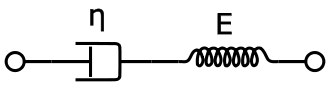
\includegraphics[width=0.5\textwidth]{figures/Maxwell-material.png}
    \caption{Schematische Darstellung des Maxwell - Materials}
    \label{fig:Maxwell-Material}
\end{figure}

Die resultierende Differentialgleichung fue;r die Schubspannung $\T$ nimmt folgende Form an:
%
\newnot{symbol:lambda}
\begin{equation}
    \label{eq:maxwellModell}
    \T + \lambda \frac{\partial\T}{\partial t}=2\eta \D
\end{equation}
Die Voraussetzung dafür ist dass das Stoffverhalten als linear angenommen wird, indem nur Verzerrungen mit hinreichend kleiner Amplitude betrachtet werden. Zusätzlich muss noch die Annahme eines exponentiell schwindenden Gedächtnisses getroffen werden, das heisst der Einfluss von Verzerrungen auf die aktuelle Spannung nimmt mit der Zeit exponentiell ab.
Wie schnell dieser Einfluss abnimmt, hängt dabei von der Relaxationszeit $\lambda$ ab.
%Wird dabei lineares Stoffverhalten vorausgesetzt indem nur Verzerrungen mit hinreichend kleiner Amplitude betrachtet werden, kann die Funktion $F$ in erster Näherung als linear betrachtet werden. Falls zusätzlich noch die Annahme eines schwindenden Gedächtnisses getroffen, das heisst der Einfluss von Verzerrungen auf die aktuelle Spannung nimmt mit der Zeit monoton ab, kann die Beziehung zwischen $\T$ und $\D$ als Integral

Eine Erweiterung dieses Modells ist das Oldroyd-B Modell, bei dem statt die partielle die kontravariante Ableitung $\overset{\nabla}{\T}$ verwendet wird:
\begin{equation}
    \label{eq:oldroydModell}
    \T + \lambda \overset{\nabla}{\T}=2\eta \D
\end{equation}
wobei
\begin{equation}
    \label{eq:upperconvectedDerivative}
    \overset{\nabla}{\T} = \frac{D}{Dt}\T-\left[ \nabla u^T\cdot \T \right]-\left[ \T\cdot \nabla u \right] 
\end{equation}
Diese Modifikation dient dazu, Drehungen und Verzerrungen des Fluides in der Differentialgleichung zu berue;cksichtigen.

Das in dieser Arbeit verwendete Modell fue;r viskoelastische Fluide muss zusae;tzlich zu der Zeitabhae;ngigkeit auch die stark scherratenabhae;ngigen Effekte berue;cksichtigen koe;nnen.\\
Dazu in der Lage ist das White-Metzner Modell. Dieses ist eine Erweiterung des Oldroyd-B Modelles, bei dem zusae;tzlich $\lambda$ und $\eta$ eine Funktion von $\gammap$ sind:
\begin{equation}
    \label{eq:whiteMetznerModell}
    \T + \lambda\left( \gammap \right) \overset{\nabla}{\T}=2\eta\left( \gammap \right) \D
\end{equation}
Dabei koe;nnen im Allgemeinen fue;r die Funktionen $\lambda$ und $\eta$ die selben Modelle wie fue;r die nicht zeitabhae;ngigen Gesetze verwendet werden.
In dieser Arbeit wurde fue;r $\eta$ das schon bewae;hrte modifizierte Herschel Bulkley Modell \eqref{eq:modHB} implementiert.\\
Fue;r die Relaxationszeit $\lambda$ wird auf Empfehlung des Rheologiespezialisten von Hilti das Carreau-Yasuda Modell verwendet:
%
\begin{equation}
    \label{eq:carreauYasuda}
    \lambda \left( \gammap \right) = \eta_{\inf} +\left( \eta_0 - \eta_{\inf} \right) \left( 1+\left( L\gammap \right)^\alpha \right)^{\frac{n_{\lambda}-1}{\alpha}}
\end{equation}
%
Die Parameter $\eta_{\inf}$, $\eta_0$, $L$, $\alpha$ und $n_{\lambda}$ sind dabei wieder materialabhae;ngig. 
%
%\subsubsection{Strukturviskosität}
%%
%\subsubsection{Viskoelastizität}
%%
%\subsubsection{Konstitutive Gesetze}
